% Overleaf-ready tuned-only results section for the WormShield paper.
% Required packages: graphicx, booktabs, amsmath

\section{Simulation and Results}
\label{sec:simulation-results}

\subsection{Experimental Setup}

We evaluate WormShield on both the AgentArena dataset described in
Section~IV and the external Here-Comes-the-AI-Worm benchmark. The
two datasets stress different aspects of worm detection. AgentArena is
designed to capture propagation through multi-step agent relays,
including copied instructions, paraphrased payloads, and partially
preserved malicious intent. Here-Comes-the-AI-Worm provides an
external benchmark that is useful for checking whether the detector
generalizes beyond the AgentArena sandbox.

For AgentArena, the original decision labels are collapsed into a
binary detection task in which \texttt{propagating} is the positive
class and \texttt{clean} and \texttt{exposed} are negative. Train,
validation, and test partitions are grouped by complete AgentArena run
so that examples from the same propagation trace cannot leak across
splits. For Here-Comes-the-AI-Worm, the official test partition is
kept unchanged and grouped development splits are constructed over
the training partition by person.

The detector studied in this section uses score-level fusion of
three branches: a surface-form similarity branch, a semantic
branch, and a payload branch. Let $s_{\mathrm{sim}}$,
$s_{\mathrm{sem}}$, and $s_{\mathrm{pay}}$ denote the normalized
branch scores. The tuned detector score is
\begin{equation}
s_{\mathrm{WG}} =
0.50 s_{\mathrm{sim}} +
0.06 s_{\mathrm{sem}} +
0.44 s_{\mathrm{pay}}.
\label{eq:wg-tuned-fusion-paper}
\end{equation}
All WormShield rows report mean $\pm$ standard deviation over five
random seeds,
\[
\{7,19,31,43,59\},
\]
with a fixed decision threshold $\tau = 0.5$.

\subsection{Cross-Dataset Detection Performance}

Table~\ref{tab:tuned-main-results} compares the tuned WormShield
detector with the published DonkeyRail summary row on both
datasets.

\begin{table*}[t]
\centering
\small
\setlength{\tabcolsep}{4pt}
\caption{Tuned WormShield comparison on AgentArena and
Here-Comes-the-AI-Worm. WormShield rows report five-seed mean
$\pm$ standard deviation. Lower is better for FPR.}
\label{tab:tuned-main-results}
\begin{tabular}{llccccccc}
\toprule
Dataset & Model & Accuracy & Precision & Recall & F1 & ROC-AUC & PR-AUC & FPR \\
\midrule
AgentArena
& DonkeyRail
& 0.7326
& 0.5339
& \textbf{0.8310}
& 0.6501
& 0.7608
& --
& 0.3436 \\
& WormShield tuned fusion
& \textbf{0.7842 $\pm$ 0.0309}
& \textbf{0.6121 $\pm$ 0.0574}
& 0.7568 $\pm$ 0.0175
& \textbf{0.6751 $\pm$ 0.0333}
& \textbf{0.8550 $\pm$ 0.0135}
& 0.7346 $\pm$ 0.0170
& \textbf{0.2041 $\pm$ 0.0455} \\
\midrule
Here-Comes-the-AI-Worm
& DonkeyRail
& 0.9806
& 0.9653
& 0.9938
& 0.9793
& 0.9816
& --
& 0.5085$^{\dagger}$ \\
& WormShield tuned fusion
& \textbf{0.9826 $\pm$ 0.0008}
& \textbf{0.9745 $\pm$ 0.0006}
& \textbf{0.9940 $\pm$ 0.0018}
& \textbf{0.9842 $\pm$ 0.0007}
& \textbf{0.9941 $\pm$ 0.0003}
& \textbf{0.9929 $\pm$ 0.0003}
& \textbf{0.0310 $\pm$ 0.0008} \\
\bottomrule
\end{tabular}

\vspace{1mm}
\parbox{0.97\textwidth}{\footnotesize
$^{\dagger}$ The published DonkeyRail FPR value for
Here-Comes-the-AI-Worm should be verified before submission because
it appears inconsistent with the other reported summary metrics.}
\end{table*}

The tuned fusion improves the overall operating point on both
datasets. On AgentArena, the largest gains appear in precision,
ROC-AUC, and FPR. Relative to DonkeyRail, accuracy rises from
0.7326 to $0.7842 \pm 0.0309$, F1 rises from 0.6501 to
$0.6751 \pm 0.0333$, and FPR drops from 0.3436 to
$0.2041 \pm 0.0455$. The only metric that does not improve is
recall, which falls from 0.8310 to $0.7568 \pm 0.0175$. This means
that on AgentArena the tuned detector is better interpreted as a
cleaner and more selective operating point rather than as a strict
recall-maximizing detector.

On Here-Comes-the-AI-Worm, the tuned fusion improves every reported
summary metric relative to the published DonkeyRail row. Accuracy
reaches $0.9826 \pm 0.0008$, F1 reaches
$0.9842 \pm 0.0007$, ROC-AUC reaches
$0.9941 \pm 0.0003$, and PR-AUC reaches
$0.9929 \pm 0.0003$. This result is important because it shows
that adding a similarity branch recovers the performance gap that
appeared when the detector relied only on semantic and payload
signals.

To provide a broader AI-Worm comparison, Table~\ref{tab:aiworm-expanded}
adds the other model families reported by the original
Here-Comes-the-AI-Worm benchmark release. Because the benchmark
reports multiple feature combinations per model family, we show the
best released row for each model by F1 on the official test split.
These added baselines are available only for AI-Worm, so they are
reported separately from the cross-dataset table above.

\begin{table*}[t]
\centering
\small
\setlength{\tabcolsep}{4pt}
\caption{Expanded Here-Comes-the-AI-Worm comparison. Decision
Stump, Logistic Regression, and Naive Bayes rows are taken from the
released benchmark result tables, using the best feature combination
per model family by reported F1. Lower is better for FPR.}
\label{tab:aiworm-expanded}
\begin{tabular}{lccccccc}
\toprule
Model & Feature setting & Accuracy & Precision & Recall & F1 & ROC-AUC & FPR \\
\midrule
Decision Stump & BLEU + METEOR
& 0.9806
& 0.9653
& 0.9938
& 0.9793
& 0.9816
& 0.5085$^{\dagger}$ \\
Logistic Regression & ROUGE-L + METEOR
& 0.9742
& 0.9523
& 0.9938
& 0.9726
& \textbf{0.9953}
& 0.0454 \\
Naive Bayes & METEOR
& 0.9734
& 0.9509
& 0.9938
& 0.9719
& 0.9950
& 0.0450 \\
WormShield tuned fusion & similarity + semantic + payload
& \textbf{0.9826 $\pm$ 0.0008}
& \textbf{0.9745 $\pm$ 0.0006}
& \textbf{0.9940 $\pm$ 0.0018}
& \textbf{0.9842 $\pm$ 0.0007}
& 0.9941 $\pm$ 0.0003
& \textbf{0.0310 $\pm$ 0.0008} \\
\bottomrule
\end{tabular}

\vspace{1mm}
\parbox{0.97\textwidth}{\footnotesize
$^{\dagger}$ The released Decision Stump FPR value for
Here-Comes-the-AI-Worm appears inconsistent with its other summary
metrics and should be verified before submission.}
\end{table*}

The expanded AI-Worm comparison shows that WormShield remains the
strongest fixed-threshold operating point among the reported model
families. It achieves the best accuracy, precision, recall, F1, and
FPR in Table~\ref{tab:aiworm-expanded}. Logistic Regression and
Naive Bayes retain slightly higher ROC-AUC, which means their score
rankings are marginally stronger when averaged across all possible
thresholds. However, at the deployed threshold $\tau = 0.5$,
WormShield gives the cleanest practical operating point, which is the
more relevant comparison for a guardrail that must actually decide
whether to block a relay in deployment.

\subsection{Branch Ablation on AgentArena}

Table~\ref{tab:tuned-agentarena-ablation} examines how the three
branches behave on AgentArena. This ablation is important because
AgentArena contains the paraphrased and multi-hop propagation patterns
that motivate WormShield in the first place.

\begin{table*}[t]
\centering
\small
\setlength{\tabcolsep}{4pt}
\caption{AgentArena branch ablation for similarity, semantic, payload,
and their combinations. Lower is better for FPR.}
\label{tab:tuned-agentarena-ablation}
\begin{tabular}{lccccccc}
\toprule
Variant & Accuracy & Precision & Recall & F1 & ROC-AUC & PR-AUC & FPR \\
\midrule
Similarity only
& 0.6890 $\pm$ 0.0260
& 0.4808 $\pm$ 0.0393
& 0.5761 $\pm$ 0.0361
& 0.5220 $\pm$ 0.0170
& 0.7387 $\pm$ 0.0126
& 0.5537 $\pm$ 0.0112
& 0.2639 $\pm$ 0.0481 \\
Semantic only
& 0.9027 $\pm$ 0.0076
& 0.8524 $\pm$ 0.0221
& 0.8108 $\pm$ 0.0200
& 0.8307 $\pm$ 0.0121
& 0.9574 $\pm$ 0.0045
& 0.9170 $\pm$ 0.0079
& 0.0587 $\pm$ 0.0094 \\
Payload only
& 0.6190 $\pm$ 0.0251
& 0.4288 $\pm$ 0.0250
& \textbf{0.8750 $\pm$ 0.0228}
& 0.5751 $\pm$ 0.0236
& 0.7377 $\pm$ 0.0216
& 0.4958 $\pm$ 0.0282
& 0.4874 $\pm$ 0.0314 \\
Similarity + Payload
& 0.7472 $\pm$ 0.0277
& 0.5592 $\pm$ 0.0503
& 0.7280 $\pm$ 0.0390
& 0.6299 $\pm$ 0.0234
& 0.8240 $\pm$ 0.0130
& 0.6769 $\pm$ 0.0213
& 0.2446 $\pm$ 0.0504 \\
Semantic + Payload
& \textbf{0.9072 $\pm$ 0.0067}
& 0.8620 $\pm$ 0.0226
& 0.8162 $\pm$ 0.0189
& \textbf{0.8381 $\pm$ 0.0114}
& \textbf{0.9582 $\pm$ 0.0056}
& 0.9192 $\pm$ 0.0063
& 0.0546 $\pm$ 0.0093 \\
Similarity + Semantic
& 0.9028 $\pm$ 0.0071
& 0.8537 $\pm$ 0.0270
& 0.8095 $\pm$ 0.0187
& 0.8305 $\pm$ 0.0116
& 0.9577 $\pm$ 0.0057
& 0.9182 $\pm$ 0.0076
& 0.0580 $\pm$ 0.0118 \\
Similarity + Semantic + Payload
& 0.9055 $\pm$ 0.0084
& \textbf{0.8624 $\pm$ 0.0248}
& 0.8092 $\pm$ 0.0223
& 0.8345 $\pm$ 0.0137
& 0.9579 $\pm$ 0.0057
& \textbf{0.9196 $\pm$ 0.0093}
& \textbf{0.0540 $\pm$ 0.0104} \\
\bottomrule
\end{tabular}
\end{table*}

The AgentArena ablation shows that semantic modeling is the dominant
signal on the propagation-heavy sandbox dataset. Similarity alone is
weak, which is expected because many malicious relays in AgentArena are
paraphrased rather than copied verbatim. Payload-only behaves very
differently: it achieves the highest recall, but does so with a very
large false-positive rate. The best F1 and ROC-AUC come from
semantic + payload, while the full three-branch model gives the
best PR-AUC and the lowest FPR. In other words, similarity is not
the main driver on AgentArena, but it still helps slightly refine the
decision boundary when added on top of semantic and payload cues.

\subsection{Branch Ablation on Here-Comes-the-AI-Worm}

Table~\ref{tab:tuned-aiworm-ablation} reports the corresponding
ablation on Here-Comes-the-AI-Worm.

\begin{table*}[t]
\centering
\small
\setlength{\tabcolsep}{4pt}
\caption{AI-Worm branch ablation for similarity, semantic, payload,
and their combinations. Lower is better for FPR.}
\label{tab:tuned-aiworm-ablation}
\begin{tabular}{lccccccc}
\toprule
Variant & Accuracy & Precision & Recall & F1 & ROC-AUC & PR-AUC & FPR \\
\midrule
Similarity only
& 0.9746 $\pm$ 0.0045
& 0.9686 $\pm$ 0.0046
& 0.9852 $\pm$ 0.0040
& 0.9769 $\pm$ 0.0041
& 0.9879 $\pm$ 0.0026
& 0.9852 $\pm$ 0.0026
& 0.0380 $\pm$ 0.0057 \\
Semantic only
& 0.9018 $\pm$ 0.0036
& 0.8988 $\pm$ 0.0024
& 0.9233 $\pm$ 0.0073
& 0.9109 $\pm$ 0.0035
& 0.9594 $\pm$ 0.0020
& 0.9587 $\pm$ 0.0027
& 0.1238 $\pm$ 0.0036 \\
Payload only
& 0.8510 $\pm$ 0.0000
& 0.9857 $\pm$ 0.0000
& 0.7366 $\pm$ 0.0000
& 0.8432 $\pm$ 0.0000
& 0.9903 $\pm$ 0.0040
& 0.9846 $\pm$ 0.0063
& 0.0127 $\pm$ 0.0000 \\
Similarity + Payload
& 0.9773 $\pm$ 0.0227
& \textbf{0.9908 $\pm$ 0.0004}
& 0.9671 $\pm$ 0.0418
& 0.9784 $\pm$ 0.0222
& \textbf{0.9953 $\pm$ 0.0003}
& \textbf{0.9932 $\pm$ 0.0002}
& \textbf{0.0106 $\pm$ 0.0003} \\
Semantic + Payload
& 0.8692 $\pm$ 0.0097
& 0.9786 $\pm$ 0.0015
& 0.7764 $\pm$ 0.0181
& 0.8657 $\pm$ 0.0113
& 0.9740 $\pm$ 0.0016
& 0.9766 $\pm$ 0.0014
& 0.0202 $\pm$ 0.0015 \\
Similarity + Semantic
& 0.9703 $\pm$ 0.0006
& 0.9548 $\pm$ 0.0013
& 0.9924 $\pm$ 0.0005
& 0.9732 $\pm$ 0.0005
& 0.9904 $\pm$ 0.0005
& 0.9897 $\pm$ 0.0004
& 0.0559 $\pm$ 0.0017 \\
Tuned fusion $(0.50, 0.06, 0.44)$
& \textbf{0.9826 $\pm$ 0.0008}
& 0.9745 $\pm$ 0.0006
& \textbf{0.9940 $\pm$ 0.0018}
& \textbf{0.9842 $\pm$ 0.0007}
& 0.9941 $\pm$ 0.0003
& 0.9929 $\pm$ 0.0003
& 0.0310 $\pm$ 0.0008 \\
\bottomrule
\end{tabular}
\end{table*}

The AI-Worm ablation tells a different story from AgentArena. Here,
similarity is already a very strong single branch, which indicates
that many positive examples preserve enough lexical or structural
overlap for surface-form evidence to remain useful. Payload-only
again acts as a high-precision but low-recall detector. The
similarity + payload pair gives the best precision, ROC-AUC,
PR-AUC, and FPR, but the tuned three-branch fusion gives the best
overall Accuracy, Recall, and F1. This is the main reason for using
the tuned fusion as the cross-dataset detector: it is not the best
branch combination for every individual metric, but it provides the
best overall balance across both datasets.

\subsection{Weight Sensitivity of the Tuned Fusion}

The weight sweep in Fig.~\ref{fig:tuned-weight-sensitivity} helps
explain why the tuned detector works well on AI-Worm. The strongest
region is consistently similarity-heavy, with a small semantic
weight and a moderate payload contribution. This matches the
ablation tables: similarity recovers broad coverage, payload keeps
the detector selective, and a small semantic contribution stabilizes
the final operating point. The selected tuned setting
$(0.50,0.06,0.44)$ lies very close to the best coarse grid point
observed in the sweep, namely $(0.50,0.05,0.45)$.

\begin{figure}[t]
    \centering
    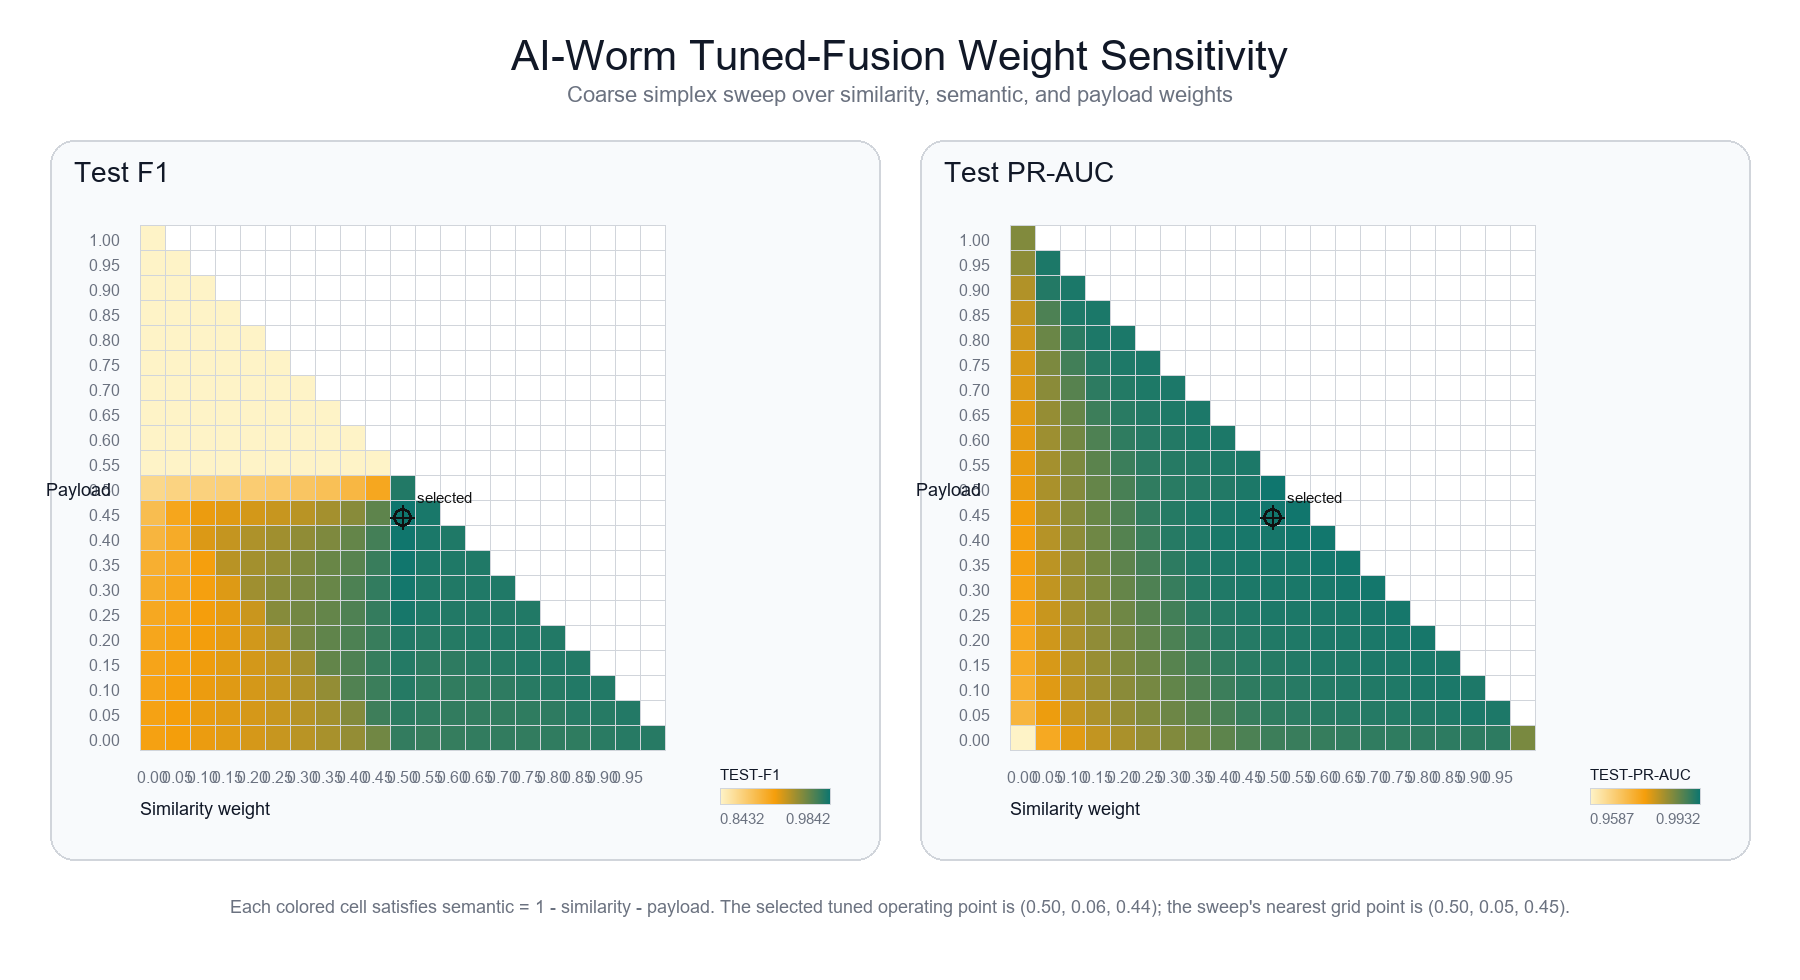
\includegraphics[width=\linewidth]{figures/wormshield-tuned-weight-sensitivity-clean.png}
    \caption{AI-Worm weight sensitivity for the tuned WormShield
    fusion. Each valid cell satisfies
    $w_{\mathrm{sem}} = 1 - w_{\mathrm{sim}} - w_{\mathrm{pay}}$.
    The selected operating point lies inside a stable
    similarity-heavy region with high test F1 and high PR-AUC.}
    \label{fig:tuned-weight-sensitivity}
\end{figure}

\subsection{Summary of Findings}

Three conclusions follow from these experiments. First, the tuned
fusion clearly improves the overall cross-dataset comparison against
the published DonkeyRail baseline. Second, AgentArena and
Here-Comes-the-AI-Worm emphasize different signals: AgentArena favors
semantic and payload evidence, whereas AI-Worm benefits much more
from similarity. Third, the tuned three-branch fusion is useful not
because every branch is equally important, but because it balances
the different failure modes of the individual branches and gives the
strongest overall detector story across the two datasets.
